%--------------------------------------------%
% Template Beamer para Apresentações da UFRN %
% by alcemygvseverino@gmail.com              %
% Baseado em MIT Beamer Template			 %
% versao 1.1								 %
% Atualizado em 14/05/2016					 %
%--------------------------------------------%
\documentclass[]{beamer}

\mode<presentation>
{
% Para definir o tema do slide
\usetheme{Berlin}
% Para difinir cores e background
\usecolortheme{ufrn}
% Para numerar as figuras
\setbeamertemplate{caption}[numbered]
	\setbeamercovered{transparent}
}

% Para alterar a linguagem do documento
\usepackage[spanish]{babel}
% Para aceitar caracteres especias deretamente do teclado
\usepackage[utf8]{inputenc}
% Para seguir as normas da ABNT de citacao e referencias
\usepackage[alf]{abntex2cite}
% Para incluir figuras
\usepackage{graphicx}
% Para melhor ajuste da posisao das figuras
\usepackage{float}
% Para ajustar as dimensoes do layout da pagina
\usepackage{geometry}
% Para formatar estrutura e informacoes de formulas matematicas
\usepackage{amsmath}
% Para incluir simbolos especiais em formulas matematicas
\usepackage{amssymb}
% Para incluir links nas referencias
\usepackage{url}
% Para incluir paginas de documentos .pdf externos
\usepackage{pgfpages}
% Para ajustar o estilo dos contadores
\usepackage{enumerate}
% Para modificar a cor do texto
\usepackage{color}
% Para incluir condicoes
\usepackage{ifthen}
% Para colocar legendas em algo que nao e float
\usepackage{capt-of}
\usepackage{hyperref}
\usepackage{algorithm,algorithmic}
\usepackage{colortbl}

%\usepackage[T1]{fontenc}
\usepackage{inconsolata}
\usepackage{listings}

\lstset{language=Java,
basicstyle=\footnotesize\tt,        % the size of the fonts that are used for the code
 breakatwhitespace=false,         % sets if automatic breaks should only happen at whitespace
 breaklines=true,                 % sets automatic line breaking
 captionpos=b,                    % sets the caption-position to bottom
 extendedchars=true,              % lets you use non-ASCII characters; for 8-bits encodings only, does not work with UTF-8
 frame=single,                    % adds a frame around the code
 language=Java,                 % the language of the code
 keywordstyle=\bf,
 showspaces=false,                % show spaces everywhere adding particular underscores; it overrides 'showstringspaces'
 showstringspaces=false,          % underline spaces within strings only
 showtabs=false,                  % show tabs within strings adding particular underscores
 tabsize=2                       % sets default tabsize to 2 spaces
}


% Título

\title[Programaci\'on 2]{Programaci\'on 2}
\subtitle{Lenguaje Java - Manejo de Archivos en GUI.}
% Data
\date{
	\today}
% Autores
\author[Eduardo Godoy]{
	Profesor: Eduardo Godoy. \\
	\vspace{0.5mm}
	\texttt{\small eduardo.gl@gmail.com}
}
% Instituto
\institute[Universidad de Valara\'iso]{

%\texttt{\normalsize eduardo.gl@gmail.com} \\
	\vspace{0.25cm}
	\texttt Escuela de Ingenier\'ia Civil Inform\'atica.\\
	\texttt Universidad de Valpara\'iso.
}
% Logo do canto inferior direito



\begin{document}

% Sumário
\frame{\titlepage}
\section[]{}
\begin{frame}{Contenido}
	\tableofcontents
\end{frame}

% excepciones
\section{Acceso a Datos}

\begin{frame}{Manejo de archivos - Archivo Secuencial}
	\begin{block}{}
	\begin{itemize}
\item Forma básica de almacenar registros en un archivos.
\item Sus registros son de similares en exstructura y tama\~no.
\item Se ordenan de forma secuencial en base a un valor de campo o atributo, en nuestro caso un ID.
\end{itemize}
\end{block}
\end{frame}


\begin{frame}{Manejo de archivos}
	\begin{itemize}
	%	\item[] crear():
\item Archivo Origen o Base: Encargado de almacenar los registros de forma persistente. Adem\'as gestiona y mantene su estado en el tiempo.
\item Archivo Auxiliar:  Encargado de dar soporte a las operaciones b\'asicas sobre el archivo origen, permitiendo hacer cambios de estado. Debido a que se emplea como medida de respaldo.
\item Las operaciones b\'asicas son los m\'etodos: crear, actualizar y eliminar.
\end{itemize}
\end{frame}

\begin{frame}{Manejo de archivos - crear()}
	\begin{itemize}
	%	\item[] crear():
\item Se recorre archivo de inicio a fin.
\item Se procede a la copia de registros desde archivo origen a archivo auxiliar
\item Por cada linea leida se guarda su id siendo este sobre escrito por el valor id de la siguiente linea procesada.
\item Cada Registro Le\'ido se almacena en el archivo axiliar.
\item Se continua con la inserci\'on del nuevo registro al final del archivo auxiliar con el ultimo id obtenido \item incrementado en 1, con esto se obtienen claves \'unicas para cada registro.
\item Se finaliza con el cipiado del archivo auxiliar al orchivo base.
\end{itemize}
\end{frame}

\begin{frame}{Manejo de archivos - actualizar()}
\begin{itemize}
%\item[] actualizar():
\item Se recorre archivo de inicio a fin.
\item Se procede a la copia de registros desde archivo origen a archivo auxiliar
 \item Por cada linea leida se comparar su id  con el id pasado por par\'ametro.
 \item De ser iguales se inserta en el archivo auxiliar el registro actualizado que viene como pa´r\'ametro, \item dejando el registro leido desde origen sin ser escrito en auxiliar.
 \item De lo contrario se siguen escribiendo los registros en el archivo auxiliar sin ser afectados por cambios.
\item Se finaliza con el cipiado del archivo auxiliar al orchivo base.
\end{itemize}
\end{frame}

\begin{frame}{Manejo de archivos - eliminar()}
\begin{itemize}
%\item[] eliminar():
\item Se recorre archivo de inicio a fin.
\item Se procede a la copia de registros desde archivo origen a archivo auxiliar
\item Por cada linea leida desde origen se compara su id  con el id pasado por par\'ametro.
\item De ser iguales ese registros se marca como nulo.
\item Cada registro Le\'ido se almacena en el archivo axiliar. excepto el que ha sido marcado como nulo.
\end{itemize}
\end{frame}

\begin{frame}{Manejo de archivos - grabar()}
\begin{itemize}
%\item[] grabar():
\item Genera una copia del archivo origen con un nombre de respaldo.
\item Toma el archivo origen y borra su contenido.
\item Escribe la cabecera del archivo en origen.
\item Recorre el archivo auxiliar leyendo cada registro.
\item Para cada registro leido desde auxiliar es escrito en origen.
	\end{itemize}
\end{frame}


% Wrappers
\section{Java Swing: Data Table}
\begin{frame}{Concepto de mantenedor}
\begin{block}{}
	%	\item[] crear():
	\begin{itemize}
		\item Interfaz de Usuario que permite administrar una base de datos mediante las operaciones de agregar, modificar y eliminar.
		\item Utilizados para  gestionar los registros almacenados en una base de datos, ya sea, una tabla de datos, un archivo u otra fuente de almacenamiento.
	\end{itemize}
\end{block}
\end{frame}

\begin{frame}{Concepto de mantenedor - Java}

	\begin{itemize}
\item Componente Java Swing cuya responsabilidad es la tabulaci\'on de datos.
\item Java provee de varios componentes swing para poder implementar de forma correcta mantenedores de fuentes de datos.
\item En general para esto se utiliza el componente JTable.
\item Se compone de Filas y Columnas.
\item Es posible seleccionar filas y extraer su valo mediante eventos de seleccion con perisfericos. Ejemplo: Mouse.
\end{itemize}
\end{frame}

\begin{frame}{Tips - Ocultamiento de Informaci\'on - Ejemplo.}
  \begin{figure}
    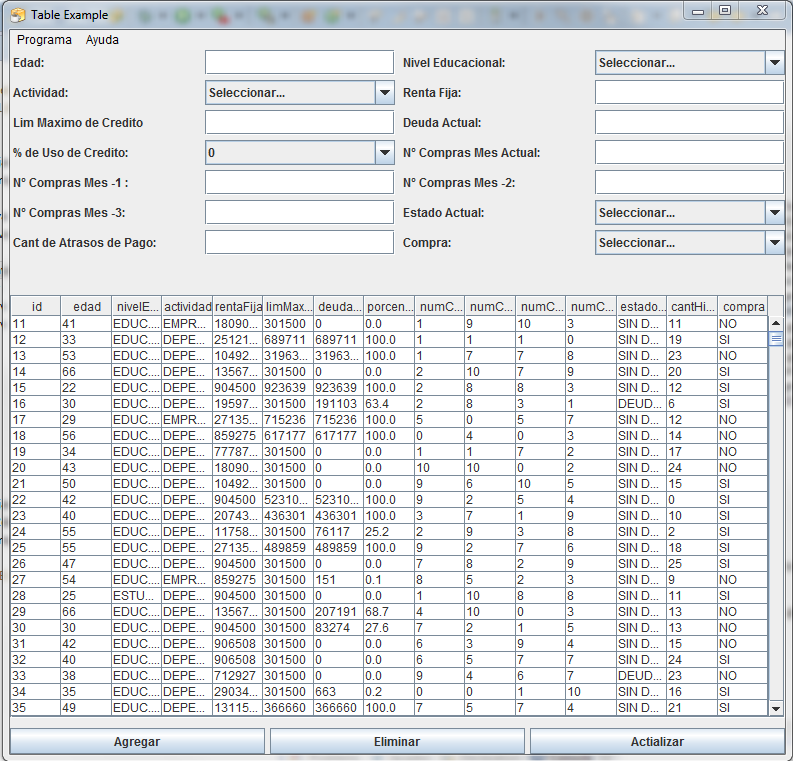
\includegraphics[scale=0.3]{figuras/DT.PNG}
  \end{figure}
\end{frame}

\begin{frame}{JTable: Instanciar Nueva}
\begin{block}{Ejemplo.}
	\lstinputlisting[language=Java,caption={},numbers=none]{resources/datatable/CrearDataTable.java}
\end{block}
\end{frame}

\begin{frame}{JTable: Agregar Regitro.}
\begin{block}{Ejemplo.}
	\lstinputlisting[language=Java,caption={},numbers=none]{resources/datatable/AddRow.java}
\end{block}
\end{frame}

\begin{frame}{JTable: Obtener Regitro.}
\begin{block}{Ejemplo.}
	\lstinputlisting[language=Java,caption={},numbers=none]{resources/datatable/GetRow.java}
\end{block}
\end{frame}

%\begin{frame}{Manejo de Excepciones - try, catch, finally}
%\begin{block}{Ejemplo.}
%\lstinputlisting[language=Java,caption={},numbers=none]{resources/excepciones/Finally.java}
%\end{block}
%\end{frame}


% apislib
%
% tips
%\section{TIPs}

\begin{frame}{Tips - Ocultamiento de Informaci\'on - Ejemplo.}
  \begin{figure}
    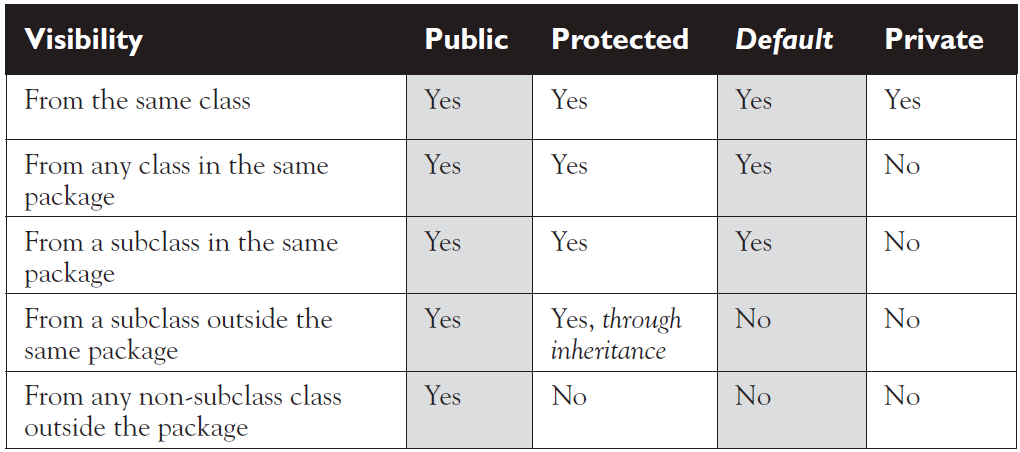
\includegraphics[scale=0.4]{figuras/ocultamiento_tabla.PNG}
  \end{figure}
\end{frame}

\begin{frame}{Tips - Casting}
	\begin{block}{Ejemplo.}
\lstinputlisting[language=Java,caption={},numbers=none]{resources/tips/Animal.java}
\end{block}
\end{frame}

\begin{frame}{Tips - Casting}
	\begin{block}{Ejemplo.}
\lstinputlisting[language=Java,caption={},numbers=none]{resources/tips/MainAnimal.java}
\end{block}
\end{frame}


% Referencias
%\include{tex/referencias/referencias}

% Agradecimentos
\section{}
%\begin{frame}{Agradecimentos}
%	Agradeço a todos.
%\end{frame}

\end{document}
